\subsection{Class Diagram}

%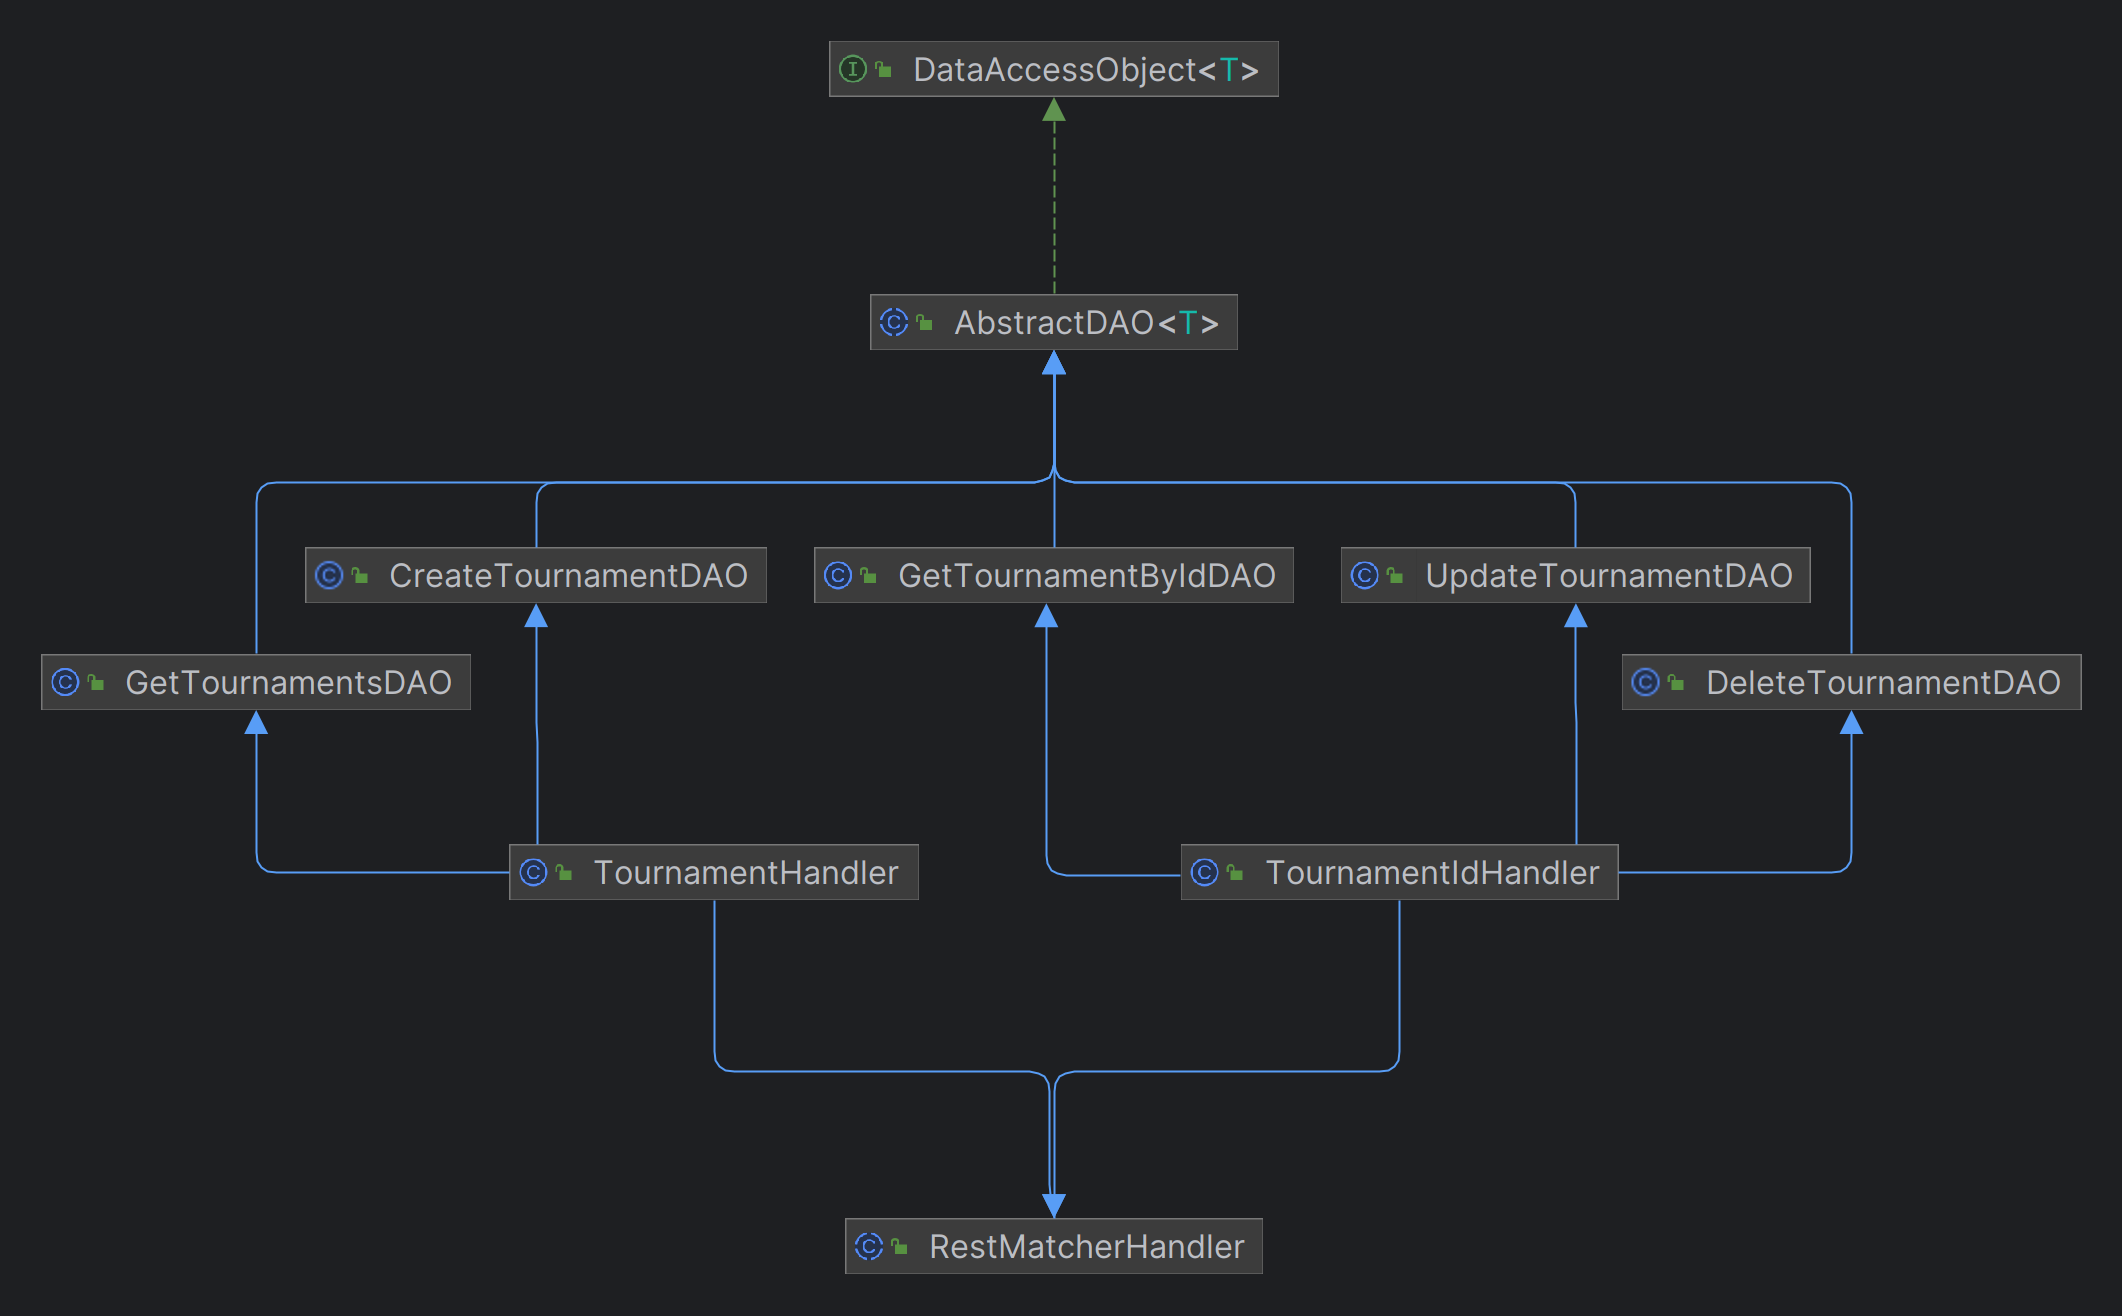
\includegraphics[]{ClassDiagram.pdf}
\textbf{IMMAGINE}

The class diagram contains (some of) the classes used to handle six types of resources: User, Tournaments, Match, Team, Player and Event. The servlets implement the doGet(), doPut(), doPost() and doDelete() methods, as sublcasses of the HttpServlet class (here omitted), depending on the cases.
Regarding the User, there are four Servlets used to handle the resource.
UserServlet handles the user-related operations, while SignupServlet, LoginServlet and LogoutServlet handles the logins in
the web application. In particular, these Servlets override doGet() and doPost() methods.
Concerning the Tournament, there are two Servlets: TournamentServlet and Home Servlet. The TournamentServlet class retrieves information about a specific tournament by its ID; the HomeServlet class is responsible for handling requests to the home page: retrieves a list of tournaments from the database and forwards the request to a JSP page (\textit{home.jsp}) for rendering.
Such Servlets implement the doGet() method.
Regarding the Match, these resources are handled through two Servlets: MatchServlet and CreateTournamentMatchesServlet. The MatchServlet class facilitates the retrieval of match details, including user authentication and authorization checks, while the CreateTournamentMatchesServlet class handles HTTP POST requests for creating matches for a tournament. It validates the URL format, checks if the user is logged in, verifies if the logged user has access to the tournament and executes a match creation job for the tournament. For this purposes, the first one overrides only the doGet() method, while the second one only the doPost() method.\\
The entities Team, Player and Event use only one Servlet each. TeamServlet overrides only the doGet() method, that can provide informations about the teams within a tournament.
PlayerServlet provides CRUD (Create, Read, Update, Delete) operations for player entities, ensuring proper authorization and error handling throughout the process.
In the end, EventServlet provides functionality for retrieving and updating event information related to a specific match.